% Unofficial University of Cambridge Poster Template
% https://github.com/andiac/gemini-cam
% a fork of https://github.com/anishathalye/gemini
% also refer to https://github.com/k4rtik/uchicago-poster

\documentclass[final]{beamer}

% ====================
% Packages
% ====================

\usepackage[T1]{fontenc}
\usepackage{lmodern}
%\usepackage[size=custom,width=120,height=72,scale=1.0]{beamerposter}
\usepackage[size=custom,width=101.6,height=76.2,scale=1.0]{beamerposter}
\usetheme{gemini}
\usecolortheme{cam}
\usepackage{graphicx}
\usepackage{booktabs}
\usepackage{tikz}
\usepackage{pgfplots}
\pgfplotsset{compat=1.14}
\usepackage{anyfontsize}
\usepackage{wrapfig}
\usepackage{multicol,multicap}
% ====================
% Lengths
% ====================

% If you have N columns, choose \sepwidth and \colwidth such that
% (N+1)*\sepwidth + N*\colwidth = \paperwidth
\newlength{\sepwidth}
\newlength{\colwidth}
%\setlength{\sepwidth}{0.025\paperwidth}
%\setlength{\colwidth}{0.3\paperwidth}
\setlength{\sepwidth}{0.06\paperwidth}
\setlength{\colwidth}{0.41\paperwidth}

\newcommand{\separatorcolumn}{\begin{column}{\sepwidth}\end{column}}

% ====================
% Title
% ====================

\title{Hierarchical Topic Modeling over Financial Documents}

\author{Ulises Hernandez \inst{1} \and Gilberto Garcia \inst{1} \and Abel Perez \inst{1} \and Nicolo Ricca \inst{1} \and Xinyu Wang \inst{1} \and Yunchen Yao \inst{1}  \and \\ Simerjot Kaur \inst{2} \and Keshav Ramani \inst{2} \and Akshat Gupta \inst{2}}



\institute[shortinst]{\inst{1} Columbia University \samelineand \inst{2} J.P. Morgan}

% ====================
% Footer (optional)
% ====================

\footercontent{
  \href{https://github.com/UlisesHdzG/Hierarchical-topic-modeling-on-financial-docs}{https://github.com/UlisesHdzG/Hierarchical-topic-modeling-on-financial-docs} \hfill
  Columbia University - DSI Capstone Project 2022, New York  %\hfill
  %\href{mailto:alyssa.p.hacker@example.com}{alyssa.p.hacker@example.com}
  }
% (can be left out to remove footer)

% ====================
% Logo (optional)
% ====================

% use this to include logos on the left and/or right side of the header:
% \logoright{
\includegraphics[height=3cm]{logos/JP-Morgan-Chase-Logo.png}}
% \logoleft{
\includegraphics[height=3cm]{logos/DSI_logo.png}}

% ====================
% Body
% ====================

\begin{document}

% Refer to https://github.com/k4rtik/uchicago-poster
% logo: https://www.cam.ac.uk/brand-resources/about-the-logo/logo-downloads
\addtobeamertemplate{headline}{}
{
    \begin{tikzpicture}[remember picture,overlay]
     \node [anchor=north west, inner sep=3cm] at ([xshift=3cm,yshift=-3cm]current page.north west)
     {
\includegraphics[height=3cm]{logos/DSI_logo.png}}; 
      \node [anchor=north east, inner sep=3cm] at ([xshift=-3.0cm,yshift=-3 cm]current page.north east)
     {
\includegraphics[height=3cm]{logos/JP-Morgan-Chase-Logo.png}};
    \end{tikzpicture}
}

\begin{frame}[t]
\begin{columns}[t]
\separatorcolumn

\begin{column}{\colwidth}

  \begin{block}{Goal (ULISES)}

    Hierarchical topic modeling is a potentially powerful instrument for determining topical structures of text collections that additionally allows constructing a hierarchy representing the levels of topic abstractness. This project focuses on exploring unsupervised learning techniques to analyze emails, from Enron data set, and generate hierarchical topics and clusters to determine the intent of the emails. 



  \end{block}

  \begin{block}{Initial Models (GAPE)}

    Briefly explain how each model work
    \begin{itemize}
      \item \textbf{LDA}
      \item \textbf{BERTopic}
      \item \textbf{LDA + BERTopic}
    \end{itemize}


  \end{block}

  \begin{block}{Topic Modeling results (YUNCHEN) }

    Show result comparison for the three models


  \end{block}

\end{column}

\separatorcolumn

\begin{column}{\colwidth}

  \begin{block}{Topic Evolution Models (XINYU and ABEL)}
    In an email, there may be more than one thread and we are interested in how the topics evolve over threads. So we analyze the topic evolution in two aspects:
    \begin{itemize}
      \item \textbf{Overall evolution (Topic Proportion)}
      \item \textbf{Evolution for each email:} we assign a topic to each email thread of an email and see how the topics evolve over the threads. The topic is assigned by \textbf{weighted-averaging} the probability that each thread belongs to a topic. If the length of current thread is short, we will put more emphasis on the previous thread's topic probability. 
    \end{itemize}
     % We use the result from our topic model to show the evolution. From our topic model, we can get the topic assignment for each email thread and the probability that each thread belongs to a topic. 

  \end{block}

  \begin{block}{Topic Evolution results (XINYU and ABEL)}

    % Show the fancy graphs and explain their interpretation. 
    % \begin{wrapfigure}[16]{L}{0.5\textwidth}
    % \begin{figure}[H]
    % \centering
    % 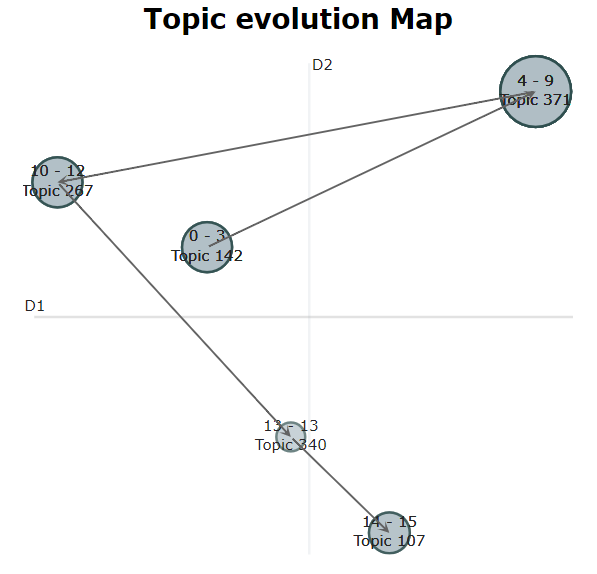
\includegraphics[width=0.5\textwidth]{bertopic_topic_evol.png}
    % \caption{Topic evolution of threads within an email }
    % \end{figure}
    % \end{wrapfigure}
    \begin{multicols}{2}
    \begin{center}
    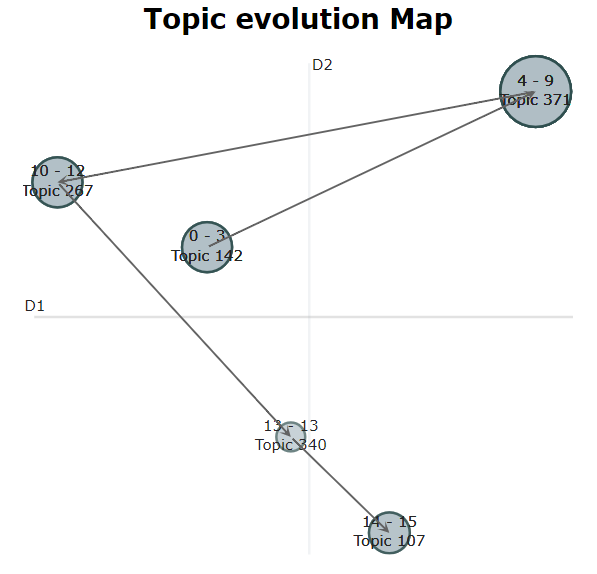
\includegraphics[width=0.5\textwidth]{bertopic_topic_evol.png}
    \mfcaption{Topic evolution of threads within an email}
    % \mfcaption{It shows how the topic evolves over threads of an email. Every circle represents a topic, the size of the circle represents the frequency of that topic and the distance between circles shows the topic similarity. The arrow can tell how the topic evolves and the text in the circle tells the topic and threads belong to this topic.}
    \label{evolution}
    \end{center}
    \begin{center}
    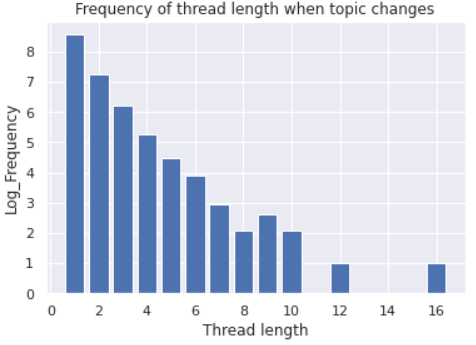
\includegraphics[width=0.3\textwidth]{bertopic_topic_change_number.png}
    \mfcaption{Topic proportion evolution over threads}
    \label{overall}
    \end{center}
    \begin{center}
    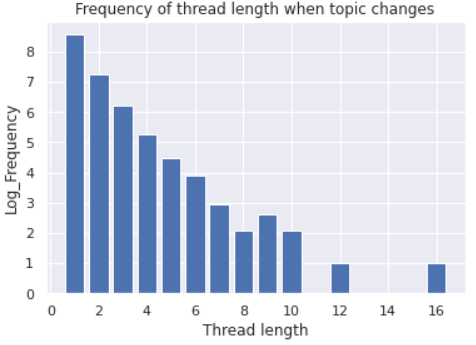
\includegraphics[width=0.3\textwidth]{bertopic_topic_change_number.png}
    \mfcaption{Number of threads for topic change}
    % \mfcaption{It shows the distribution of experiencing how many threads will the topic changes in an email. We can find that topic usually changes right after the previous email. And under most situations, the topic will change within 7 threads.}
    \label{num}
    \end{center}
\end{multicols}
    Figure \ref{evolution} shows how the topic evolves over threads of an email. Every circle represents a topic, the size of the circle represents the frequency of that topic and the distance between circles shows the topic similarity. The arrow can tell how the topic evolves and the text in the circle tells the topic and threads belong to this topic. In this example, we can 
    
    Figure \ref{overall} shows
    
    Figure \ref{num} shows the distribution of experiencing how many threads will the topic changes in an email. We can find that topic usually changes right after the previous email. And under most situations, the topic will change within 7 threads.

    % \begin{figure}[H]
    %     \centering
    %     \subfigure[拉式平滑]{
    %     \includegraphics[width=4cm,height=4cm]{change2.JPG}
    %     }
    %     \subfigure[窗口Sinc平滑]{
    %     \includegraphics[width=4cm,height=4cm]{change.JPG}
    %     }
    %     \caption{平滑方法对比}
    % \end{figure}
  \end{block}

  \begin{block}{Next Steps (NICOLO)}
      \begin{itemize}
          \item \textbf{Hierarchical LDA (HLDA):} Using the same principles as LDA, it tries to construct topic trees on multiple levels. This is based on the concept of the nested Chinese restaurant process. It has a high complexity, therefore it takes a lot of time and software to run it. 
          \item \textbf{Comparison between HLDA and H-Bertopic}
        \end{itemize}
    
    % BERTopic uses topic‐term matrix (c‐TF IDF) representations. The smaller the distance between two c‐TF‐IDF representations, the more similar we assume they are. Using this way of clustering and merging, it is possible to build a topic tree.

  \end{block}
  
%   \begin{block}{References if space permit (NICOLO)}
%     Include relevant references from first progress report and others Xinyu and Yunchen used for Topic evolution and LDA+BERTopic.
%   \end{block}
    
    


\end{column}

\separatorcolumn
\end{columns}
\end{frame}

\end{document}
